\chapter{Background: The mind as a dynamical system}\label{chap:background1}

\section{The set-up}

The set of equations $F$ defines an algebraic set = \textbf{the world}:
\begin{equation}
F(x) = 0 .
\end{equation}
The objective of an intelligent agent is to learn $F$.

We have the function $f$ performing \textbf{prediction} of the immediate future:
\begin{equation}
\boxed{\mbox{current state}} \quad x_t \stackrel{f}{\mapsto} x_{t+1} \quad \boxed{\mbox{next state}} \;.
\end{equation}

In an infinitesimal sense, we can see $f$ as a \textbf{differential equation} describing the \textbf{world trajectory}:
\begin{equation}
\dot{x} = f(x) .
\end{equation}
So $F$ is the \textbf{solution} to this differential equation.

It seems that $F$ and $f$ are more or less equivalent ways to describe the world.

Logic can be turned into some form of algebra, and this algebra can be used to express either $F$ or $f$.  Perhaps both ways are feasible, or even mixing the two.

What does it mean to use logic to express $F$ or $f$?

Go back to a physics example, the parabolic trajectory of a canon ball:
\begin{equation}
\vcenter{\hbox{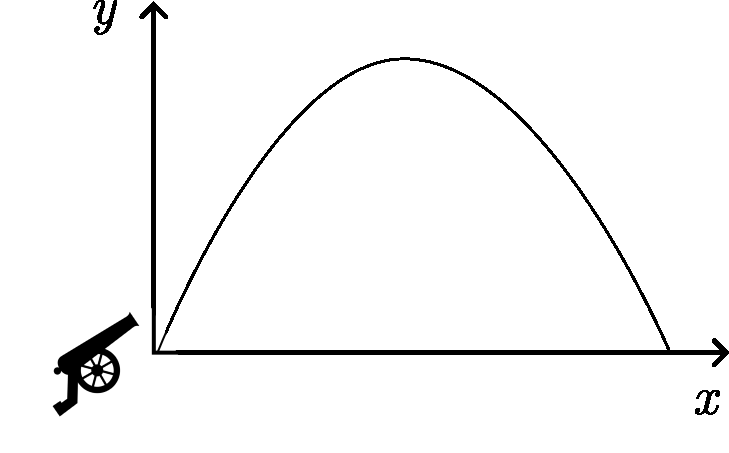
\includegraphics[scale=0.7]{canonball-parabola.png}}}
\end{equation}
The parabola is given by the quadratic equation from high school:
\begin{equation}
F(x) = 0 \qquad F(x) = ax^2 + bx + c
\end{equation}
but the trajectory can also be described by the physics equation parameterized by time $t$:
\begin{equation}
\dot{\mathbf{x}} = f(\mathbf{x}) = (v_x, v_y) = (v^0_x , -gt + v^0_y) .
\end{equation}
This parametric form is not unique.  For example, another way is for the point $\mathbf{x}$ to move with uniform speed along the trajectory.

Note that the trajectory above is qualitatively the same as a ``thought trajectory'' in cognitive space.  One intuitive way to visualize cognitive trajectories is via the example of a chess game tree:
\begin{equation}
\vcenter{\hbox{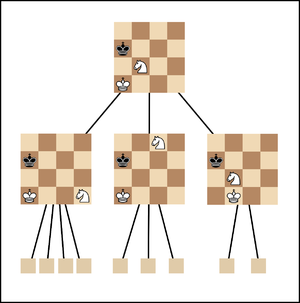
\includegraphics[scale=0.7]{chess-game-tree.png}}}
\end{equation}

$f(x)$ is the functional form we want, as it contains information about the ``interestingness'' of deduced conclusions.

Are our equations in Table \ref{table:formulas} describing $F$ or $f$?  

An intuitive idea:  state = facts = grounded equations, rules = quantified equations.  So the equations are modeling $f$.  This exposed a problem of classical AI that I have not paid too much attention to:  the selection of interesting conclusions.  It's hard to \textbf{enumerate conclusions}, let alone to rate their interestingness.

